\documentclass[a4paper,10pt]{article}

\usepackage[utf8]{inputenc}
\usepackage[english]{babel}
\usepackage[T1]{fontenc}
\usepackage{mathpazo} %http://www.ctan.org/tex-archive/fonts/mathpazo
\usepackage{stmaryrd} %http://www.ctan.org/pkg/stmaryrd
\usepackage{amsmath} %http://www.ctan.org/pkg/amsmath
\usepackage{amssymb}
\usepackage{mathrsfs}
\usepackage{subfig}

\usepackage{cite}

\usepackage{amsthm} %http://www.ctan.org/pkg/amsthm
\usepackage{proof}
\usepackage{algorithm2e}

\usepackage[colorlinks=true]{hyperref} %http://www.ctan.org/tex-archive/macros/latex/contrib/hyperref/
\hypersetup{urlcolor=black,linkcolor=black}
\usepackage{footmisc} %http://www.ctan.org/tex-archive/macros/latex/contrib/footmisc

\usepackage{enumerate}
\usepackage{ulem} %http://www.ctan.org/tex-archive/macros/latex/contrib/ulem
\normalem
\usepackage{cancel} %http://www.ctan.org/tex-archive/macros/latex/contrib/cancel

\usepackage{fullpage} %http://www.ctan.org/tex-archive/macros/latex/contrib/preprint/
\setlength{\parindent}{0pt}
\setlength{\parskip}{\medskipamount}

\usepackage{pgffor}
\usepackage{tikz}
\usetikzlibrary{arrows,shapes.arrows, chains, positioning, automata, graphs, decorations.pathreplacing}

%\usepackage[ruled,vlined,french]{algorithm2e}
%\providecommand{\SetAlgoLined}{\SetLine}
%\providecommand{\DontPrintSemicolon}{\dontprintsemicolon}

%\usepackage{forest}
\usepackage{comment} %http://www.ctan.org/tex-archive/macros/latex/contrib/comment
\usepackage{multirow} %http://www.ctan.org/tex-archive/macros/latex/contrib/multirow
\usepackage{diagbox} %http://www.ctan.org/tex-archive/macros/latex/contrib/diagbox

\usepackage{textcomp} %http://www.ctan.org/pkg/textcomp

\usepackage{listings} %http://www.ctan.org/tex-archive/macros/latex/contrib/listings/
\lstset{numbers=left,language=Caml}

\usepackage{boiboites}
\newboxedtheorem[boxcolor=orange, background=blue!5, titlebackground=blue!20,
titleboxcolor = black]{theo}{Theorem}{compteurTh}
\newboxedtheorem[boxcolor=orange, background=blue!5, titlebackground=blue!20,
titleboxcolor = black]{defi}{Definition}{compteurDef}

\newcounter{ThComp}
\newcounter{DefComp}

\newboxedtheorem[boxcolor=red, background=red!5, titlebackground=red!50,titleboxcolor = black]{theoreme}{Th\'{e}or\`{e}me}{TheC}
\newboxedtheorem[boxcolor=orange, background=orange!5, titlebackground=orange!50,titleboxcolor = black]{definition}{D\'{e}finition}{DefC}
\newboxedtheorem[boxcolor=blue, background=blue!5, titlebackground=blue!20,titleboxcolor = black]{proposition}{Proposition}{ProC}
\newboxedtheorem[boxcolor=cyan, background=cyan!5, titlebackground=cyan!20,titleboxcolor = black]{corollaire}{Corollaire}{CorC}
\newboxedtheorem[boxcolor=black, background=black!0, titlebackground=black!20,titleboxcolor = black]{remarque}{Remarque}{RemC}
\newboxedtheorem[boxcolor=green!70!black, background=green!70!black!5, titlebackground=green!70!black!30,titleboxcolor = black]{notation}{Notation}{NotC}
\newboxedtheorem[boxcolor=yellow, background=yellow!0, titlebackground=yellow!30,titleboxcolor = black]{exemple}{Exemple}{ExeC}
\newboxedtheorem[boxcolor=magenta, background=magenta!5, titlebackground=magenta!30,titleboxcolor = black]{lemme}{Lemme}{LemC}

\newcommand{\ra}{\rightarrow}
\newcommand{\la}{\leftarrow}


\newcommand{\RR}{\mathbb{R}}
\newcommand{\ZZ}{\mathbb{Z}}
\newcommand{\Ztwo}{\mathbb{Z}^{2}}
\newcommand{\NN}{\mathbb{N}}
\newcommand{\PP}{\mathbb{P}}
\newcommand{\EE}{\mathbb{E}}
\newcommand{\IE}{\mathbb{E}}
\newcommand{\IR}{\mathbb{R}}
\newcommand{\IZ}{\mathbb{Z}}
\newcommand{\IN}{\mathbb{N}}
\newcommand{\IP}{\mathbb{P}}

\newcommand{\cF}{\mathcal{F}}
\newcommand{\ck}{\mathcal{K}}
\newcommand{\cL}{\mathcal{L}}
\newcommand{\cN}{\mathcal{N}}
\newcommand{\cNU}{\mathcal{NU}}
\newcommand{\A}{\mathcal{A}}
\newcommand{\B}{\mathcal{B}}
\newcommand{\F}{\mathcal{F}}
\renewcommand{\L}{\mathcal{L}}
\newcommand{\N}{\mathcal{N}}

\newcommand{\ens}[1]{\left\{ #1 \right\}}
\newcommand{\set}[1]{\left\{ #1 \right\}}
\renewcommand{\leq}{\leqslant}
\renewcommand{\geq}{\geqslant}
\renewcommand{\le}{\leqslant}
\renewcommand{\ge}{\geqslant}
\newcommand{\cplx}[1]{\mathcal O \left( #1 \right)}
\newcommand{\floor}[1]{\left \lfloor #1 \right \rfloor}
\newcommand{\ceil}[1]{\left\lceil #1 \right\rceil}
\newcommand{\brackets}[1]{\left\llbracket #1 \right\rrbracket}
\newcommand{\donne}{\rightarrow}
\newcommand{\gives}{\rightarrow}
\newcommand{\dans}{\to}
\newcommand{\booleen}{\set{0,1}^*}
\newcommand{\eps}{\varepsilon}
\renewcommand{\implies}{~\Rightarrow~}
\newcommand{\tildarrow}{\rightsquigarrow}
\newcommand{\blank}{\texttt{\char32}}
\newcommand{\trans}[1]{\xrightarrow{#1}}
\newcommand{\rules}[1]{\xrightarrow{#1}}
\newcommand{\todo}[1]{\Large\textcolor{red}{#1}\normalsize}
\newcommand{\argmin}{\text{argmin}}
\newcommand{\rainbowdash}{\vdash}
\newcommand{\notrainbowdash}{\nvdash}
\newcommand{\rainbowDash}{\vDash}
\newcommand{\notrainbowDash}{\nvDash}
\newcommand{\Rainbowdash}{\Vdash}
\newcommand{\notRainbowdash}{\nVdash}
\newcommand{\bottom}{\bot}

%TD/TP
\newenvironment{answer}{\color{blue}}{}


%EvalPerf
\newcommand{\Var}{\text{Var}}
\newcommand{\prob}[1]{\PP\left( #1 \right)}
\newcommand{\esp}[1]{\EE\left( #1 \right)}


%SystDist
\newcommand{\Receive}{\texttt{Receive~}}
\newcommand{\Send}{\texttt{Send~}}


%Preuves
\newcommand{\betaeq}{=_\beta}
\newcommand{\betared}{\vartriangleright_\beta}
\newcommand{\parabetared}{\vartriangleright_{||\beta}}
\newcommand{\Ackermann}{\A}


%Cplx
\newcommand{\Time}{\textsc{Time}}
\newcommand{\TIME}{\textsc{Time}}

\newcommand{\dtime}{\textsc{DTime}}
\newcommand{\dTime}{\textsc{DTime}}
\newcommand{\DTime}{\textsc{DTime}}

\newcommand{\ntime}{\textsc{NTime}}
\newcommand{\nTime}{\textsc{NTime}}
\newcommand{\NTime}{\textsc{NTime}}

\renewcommand{\P}{\textsc{P}}

\newcommand{\pTime}{\textsc{PTime}}
\newcommand{\PTime}{\textsc{PTime}}

\newcommand{\NP}{\textsc{NP}}

\newcommand{\npTime}{\textsc{NPTime}}
\newcommand{\NPTime}{\textsc{NPTime}}

\newcommand{\EXP}{\textsc{Exp}}
\newcommand{\expTime}{\textsc{Exp}}
\newcommand{\ExpTime}{\textsc{Exp}}
\newcommand{\EXPTime}{\textsc{Exp}}

\newcommand{\Space}{\textsc{Space}}

\newcommand{\dSpace}{\textsc{DSpace}}
\newcommand{\DSpace}{\textsc{DSpace}}


\newcommand{\nSpace}{\textsc{NSpace}}\newcommand{\NSpace}{\textsc{NSpace}}

\newcommand{\pSpace}{\textsc{PSpace}}
\newcommand{\PSpace}{\textsc{PSpace}}

\newcommand{\npSpace}{\textsc{NPSpace}}
\newcommand{\NpSpace}{\textsc{NPSpace}}
\newcommand{\NPSpace}{\textsc{NPSpace}}

\newcommand{\SpaceTM}{\textsc{SpaceTM}}

\newcommand{\nL}{\textsc{NL}}
\newcommand{\NL}{\textsc{NL}}

\newcommand{\LL}{\textsc{L}}

\newcommand{\coNP}{co\text{-}\textsc{NP}}

\newcommand{\conL}{co\text{-}\textsc{NL}}
\newcommand{\coNL}{co\text{-}\textsc{NL}}

\newcommand{\npc}{\text{\textit{NP-C}}}

\newcommand{\PH}{\textsc{PH}}

\newcommand{\TISP}{\textsc{TISP}}

\newcommand{\Size}{\textsc{Size}}
\newcommand{\SIZE}{\textsc{Size}}





\title{A binary shape indexing/retrieval system}
\author{
    William \textsc{Aufort}\\
    Marc \textsc{Chevalier}
}
\date{\today}

\begin{document}
\maketitle

\section*{Introduction}

\subsection*{General introduction}

The objective of this project is to design a binary shape indexing system. Given a database of binary shapes (PGM files) associated to different classes, and a binary image, the goal is to find the class whch correspond the most to the image. In this document, we present and explain our main ideas to solve the problem and our implementation choices.

\subsection*{The database used}

% TODO Quelques mots sur la base de données, le type d'images (noir & blanc, type d'objets --> difficulté, ...)

\section{Granulometric analysis applied to shape indexing}

\subsection{Basic ideas}

When we are watching images, to associate them to concepts, we use our knowledge of these concepts. For example, an apple is a quite circular object with sometimes a stalk and leaves, a camel is a mammal with one or two humps, etc. Basically, for organic objects, we use a kind of segmentation caracterisation to identify the concepts: we recover it by identify its different parts.

A famous tool used in volumetric analysis to determine segmentation is the \textbf{granulometric function}. Indeed, it plays an important role for shape description, what we want exactly to do.

\begin{defi}[Granulometric function]
Let $\mathcal{X}$ be a binary shape in $\Ztwo$. We denoted by $B(c,r)$ the euclidean ball with center $c \in \Ztwo$ and radius $r \in \RR$. We define the granulometric function $g_{\mathcal{X}}$ on $\mathcal{X}$ by :

$$ g_{\mathcal{X}}(x) = \operatorname{max} \left\{ r | \exists c \in \mathcal{X}, x \in B(c,r) \wedge B(c,r) \subseteq \mathcal{X} \right\} $$ 
\end{defi}

In other words, we are looking for the radius of the greatest ball included in the shape $\mathcal{X}$ which contains our point $x$.

If we plot the granulometry function on a 2D shape in the database, we can observe that the different values of the granulometric function correspond to the different "parts" of the object. An example is given on figure \ref{apple-granulo}.

\begin{figure}[!ht]
    \centering
    \subfloat{
        \label{apple-granulo:1}   
        
\includegraphics[height=175pt]{images/apple-1}
    }
    \qquad\qquad\qquad
    \subfloat{
        \label{apple-granulo:2}
        \includegraphics[height=175pt]{images/apple-1-granulo}
    }
    \caption{The granulometric function illustrated in this apple image. We can easily distinguish the different natural parts of the apple using the granulometric function.}
    \label{apple-granulo}
\end{figure}

We can use the granulometric function to compare two images. To do this, we can see the granulometric function as a distribution of the radius of the maximal balls over the object $\mathcal{X}$, which can be describes for examples with histograms like those we use in statistics. Compare two images remains to compare two histograms, so we have to define a distance between histograms.

\subsection{Advantages}

\subsubsection{Invariant by translation, rotation and symmetry}

The invariance with respect to translation, rotation and symmetry is an important property. But we have to be a little bit more precise:

\begin{theo}[Invariance by translation]
	Let $\mathcal{X}$ be a binary shape in $\Ztwo$. Let $\vec{t} \in \Ztwo$ be a vector of translation, and let $\mathcal{X}_{t} = \left\{ x + \vec{t}, x \in \mathcal{X} \right\}$. Then :
	
	$$ \forall x \in \mathcal{X}_{t}, g_{\mathcal{X}_{t}}(x) = g_{\mathcal{X}}(x-\vec{t}) $$
\end{theo}

In other words, there is a trivial isomorphism between the two images $\mathcal{X}$ and  $\mathcal{X}_t$ seen as unions of balls. With this remark, the proof of the theorem is completely trivial.

But the same result for rotations is not completely trivial. If we take a rotation of any angle, one can imagine that the pixels of the image, after the rotation, don't match exactly with points in $\Ztwo$, because of the trigonometric functions implied during the process. The same behaviour occurs if we consider symmetries with respect to any line or center.

Nonetheless, intuitively if there exists some modifications in the granulometric function, they are not going to be very large in some sense.

% TODO : See if we can quantify the difference between the two.

\subsection{Disadvantages}

\subsubsection{Geometrical objects with perturbations}

Some of the classes are defined by the basic geometrical object they refers to. For example, the object presented in the figure \ref{device9-6}, as all the elements in the class \texttt{device9}, are very close to a ball, excepted that they are crossed by some perturbating element (in the figure it's a line). The problem on such images is that that king of noise perturbate a lot the output of the granulometric function, as we can see in the figure \ref{device9-6}.

\begin{figure}[!ht]
    \centering
    \subfloat{
        \label{device9-6:1}
        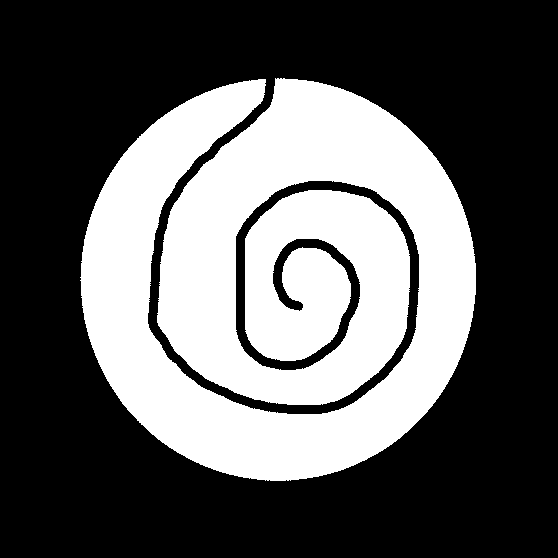
\includegraphics[height=175pt]{images/device9-6-object}
    }
    \qquad\qquad\qquad
    \subfloat{
        \label{device9-6:2}
        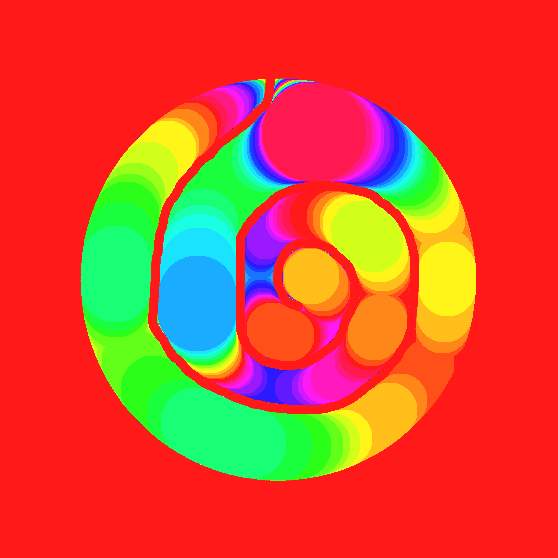
\includegraphics[height=175pt]{images/device9-6-granulo}
    }
    \caption{The granulometric function is very perturbated on this geometrical object crossed by a curve.}
	\label{device9-6}
\end{figure}

\subsubsection{Loss of spatial information}

% TODO dire quelque chose ici, voir une ouverture sur d'autres methodes (notamment les papiers que l'on a regardé)


\subsection{Implementation}

The general idea of the algorithms that computes the granulometric function is to get a quite good set of candidate balls. A ball included in the image is a candidate ball if it must have a contribution on the granulometric function of a point of the image. Indeed, most of the complexity of the algorithm leads on the iterator over those balls in order to compute the maximal radius for each point. 

We present two algorithms. The first one is quite naive and have been implemented first. It uses only the distance transformation (DT). The second one, clorer to the medial axis concept, is an optimization where we drastically reduce the number of candidate balls to scan.

\subsubsection{Naive algorithm : Distance Transformation}

We recall the definition of the Distance Transformation saw during the class :

\begin{defi}[Distance transformation]
Let $\mathcal{X}$ be a binary shape in $\Ztwo$. If $p$ is a point of $\mathcal{X}$, we called the Distance transformation at $p$, denoted by $DT(p)$, the smallest distance to the border of the image :
$$ DT(p) = \underset{q \in \widetilde{\mathcal{X}}}{min} \quad d(p,q) $$
\end{defi}

$DT(p)$ represents the maximum radius of a ball containing $p$, included in $\mathcal{X}$. We are interested in it because of this trivial result :

\begin{theo}[]
	For all $p \in \mathcal{X}$, for all $r$ such that $B(p,r) \subset \mathcal{X}$, we have :
		$$ B(p,r) \subset B(p,DT(p))$$
\end{theo}

With this result, we can restrict the number of balls to scan to $\cplx{\left| \mathcal{X} \right|}$. Indeed, we can consider only the balls $\set{B(p,DT(p)), p \in \mathcal{X}}$, because of the other balls are included in some of those ones.

Once we have computed the Distance Transformation, the algorithm to compute the granulometric function works as follows:

\IncMargin{1em}
\begin{algorithm}
\ForEach{point $p \in \mathcal{X}$}{
    Create a ball centered at $p$ with radius $DT(p)$\;
    \ForEach{point $q$ in this ball}{
        \If{$g(y) \leq DT(p)$}{
			$g(y) \leftarrow DT(p)$\;
		}
	}
}
\caption{Naive algorithm to compute the granulometric function $g$}
\label{algo-naive}
\end{algorithm}

\section{How to deal with noise: choices and implementation}

An important aspect of the project is to deal with image which can be potentially noised.

We were interested in deleting specular noise. Our choice is to implement a binomial filter saw during the course. This filter, used essentially for smoothing grayscale images, erases the potential specular noise on the image. If the image is not noisy, the experiment show that the initial image is not modified. The initial filter (i.e. for a grayscale image) is :

\setcounter{MaxMatrixCols}{3}
\[ F = \quad \frac{1}{16} \begin{pmatrix}
1 & 2 & 1 \\
2 & 4 & 2 \\
1 & 2 & 1
\end{pmatrix}\]

In the grayscale output image, we only keep the pixels with intensity greater than $8 \times 255$, where $8$ represents half of the sum of the weights in the filter ($16$ here) and $255$ the intensity for the white part of the image (i.e. the final object we keep). For more simplicity, we don't keep the $255$ factor, since the only possible intensity values in the input image are $0$ and $255$.

We give the simplier implementation of the filter in the file \texttt{deleteNoise.cpp}. One could improve it, for example using the fact that this filter is separable.

\end{document}
